\documentclass[12pt, openright, a4paper, brazil, openany, oneside]{abntex2}

\usepackage{times}		
\usepackage[T1]{fontenc}	
\usepackage[utf8]{inputenc}	
\usepackage{indentfirst}	
\usepackage{color}			
\usepackage{graphicx}		
\usepackage{microtype} 		
\usepackage{multicol}
\usepackage{multirow}
\usepackage{lipsum}				
\usepackage[brazilian,hyperpageref]{backref}

\newtheorem{teo}{Teorema}
	 
\usepackage[alf]{abntex2cite}
\renewcommand{\backrefpagesname}{Citado na(s) página(s):~}
\renewcommand{\backref}{}
\renewcommand*{\backrefalt}[4]{
	\ifcase #1 %
		Nenhuma citação no texto.%
	\or
		Citado na página #2.%
	\else
		Citado #1 vezes nas páginas #2.%
	\fi}%
\titulo{Uma bissetriz paralela aplicada na construção triangular}
\autor{Sérgio Luís Soares Almeida \\ Matrícula 18/0006410}
\local{Brasília}
\data{14 de Novembro de 2018}
\instituicao{%
  Universidade de Brasília -- UnB
  \par
  Departamento de Matemática
  \par
 PROFMAT}
\tipotrabalho{Estudo de Artigo}

\definecolor{black}{RGB}{0.0,0.0,0.0}


\makeatletter

\preambulo{Estudo do artigo An Angle Bisector Parallel Applied to
Triangle Construction publicado em 13 de julho de 2009 disponível no endereço http://forumgeom.fau.edu/FG2009volume9/FG200915.pdf}

\hypersetup{pdftitle={\@title}, pdfauthor={\@author}, pdfsubject={\imprimirpreambulo}, pdfcreator={LaTeX with abnTeX2}, pdfkeywords={abnt}{latex}{abntex}{abntex2}{relatório técnico}, colorlinks=true, linkcolor=black, citecolor=black, filecolor=black, urlcolor=black, bookmarksdepth=4}
\makeatother

\setlength{\parindent}{1.3cm}


\setlength{\parskip}{0.2cm}  


\makeindex

\begin{document}


\selectlanguage{brazil}


\frenchspacing 


\imprimircapa

\imprimirfolhaderosto*
\ABNTEXchapterfont

\pdfbookmark[0]{\contentsname}{toc}
\tableofcontents*
\cleardoublepage
\textual

\chapter*[Introdução]{Introdução}
\addcontentsline{toc}{chapter}{Introdução}


Neste estudo construiremos o círculo de nove pontos e através de um deles (Ponto de Euler) provaremos um teorema que descreve uma linha paralela a uma bissetriz de um triângulo passando pelo ponto médio do lado oposto. Nós então aplicaremos este teorema para a solução de quatro problemas de construção de triângulo.

% \let\clearpage\relax


\chapter{Pontos de Euler}

Neste capítulo iremos construir o círculo de nove pontos encontrados em um triângulo qualquer. O círculo de nove pontos é o círculo que intersecta o triângulo em pelo menos seis pontos e mais três pontos nos segmentos relativos a altura entre os vértices do triângulo e os seus lados, sendo esses últimos chamados de pontos de Euler.

Para esta construção iremos usar as seguintes notações:

\begin{itemize}
\item $\triangle ABC$ é o triângulo cujos vértices são, respectivamente $A$, $B$, e $C$.
\item O segmento $BC$ será o lado $a$, o segmento $AC$ será o lado $b$ e o segmento $AB$ será o lado $c$.

\begin{figure}[h]

    \center

    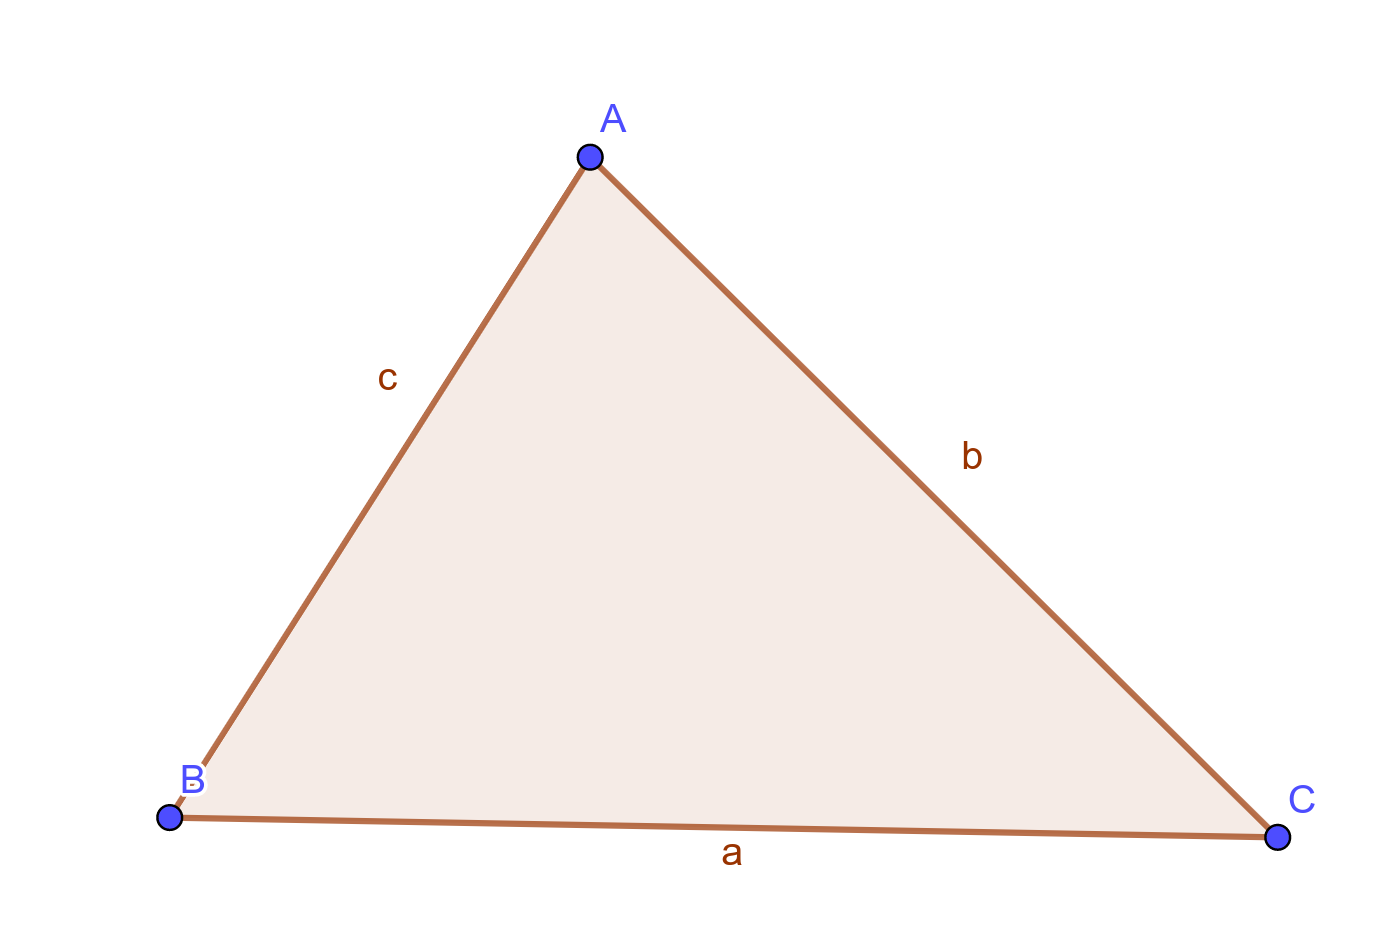
\includegraphics[width=8cm]{triangulo1.png}
    \caption{Triângulo \label{tria1}}
    
\end{figure}

\item $D$, $E$, e $F$ são os pés das alturas relativas aos lados $a$, $b$ e $c$ respectivamente.


\end{itemize} 


\section{Construindo o Círculo}

Considere o $\triangle ABC$ conforme a figura \ref{tria1} e nele traçamos as alturas relativas aos seus vértices, encontrando os pontos $D$, $E$, e $F$. Esses pontos são chamados de pés das alturas relativas.

\newpage

Considere agora o triângulo $\triangle DEF$ conforme a figura \ref{tria2} 

\begin{figure}[h]

    \center

    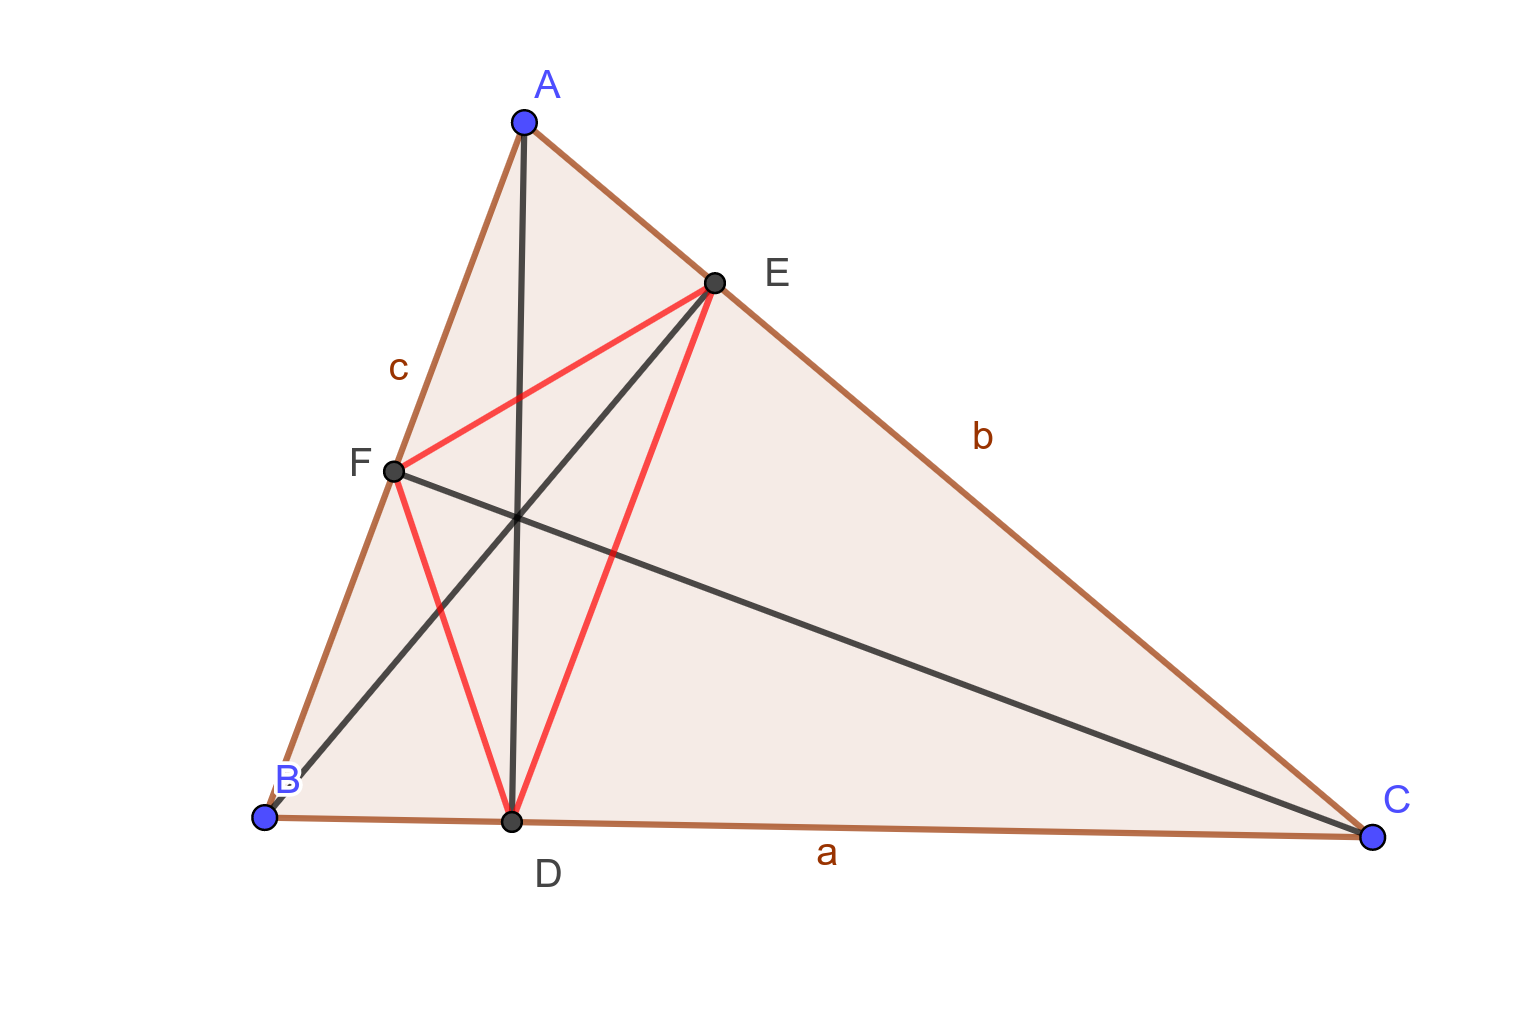
\includegraphics[width=6.9cm]{triangulo2.png}
    \caption{Alturas relativas e $\triangle DEF$ \label{tria2}}
    
\end{figure}

Vamos construir o círculo circunscrito neste triângulo e, para isso, devemos encontrar o seu circuncentro, pois este será o centro desse círculo.

Tracemos as mediatrizes referentes aos segmentos $DE$ e $EF$. O ponto de intersecção desses segmentos será o circuncentro e o raio do círculo circunscrito será a distância desse ponto a qualquer dos vértices do $\triangle DEF$.

\begin{figure}[h]

    \center

    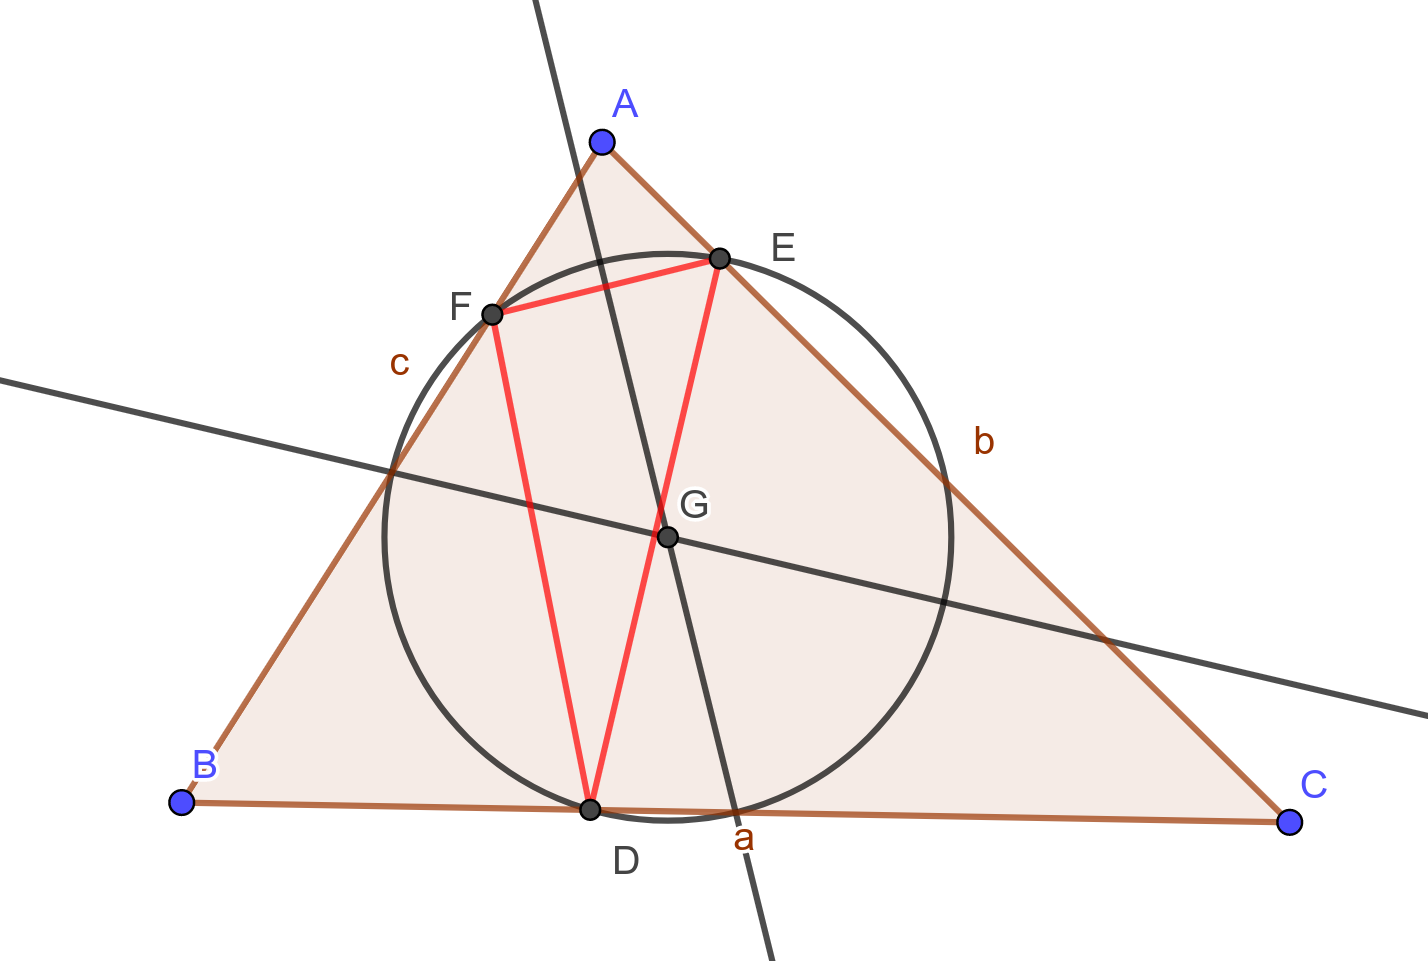
\includegraphics[width=6.9cm]{triangulo3.png}
    \caption{Alturas relativas e $\triangle DEF$ \label{tria3}}
    
\end{figure}

Este círculo terá 6 pontos de intersecção com o $\triangle ABC$: $D$, $E$, $F$, $H$, $I$ e $J$ e mais três pontos de intersecção com as alturas relativas aos lados desse triângulo: $K$, $L$ e $M$. Esses últimos três pontos são chamados de \textit{pontos de Euler}.

\begin{figure}[h]

    \center

    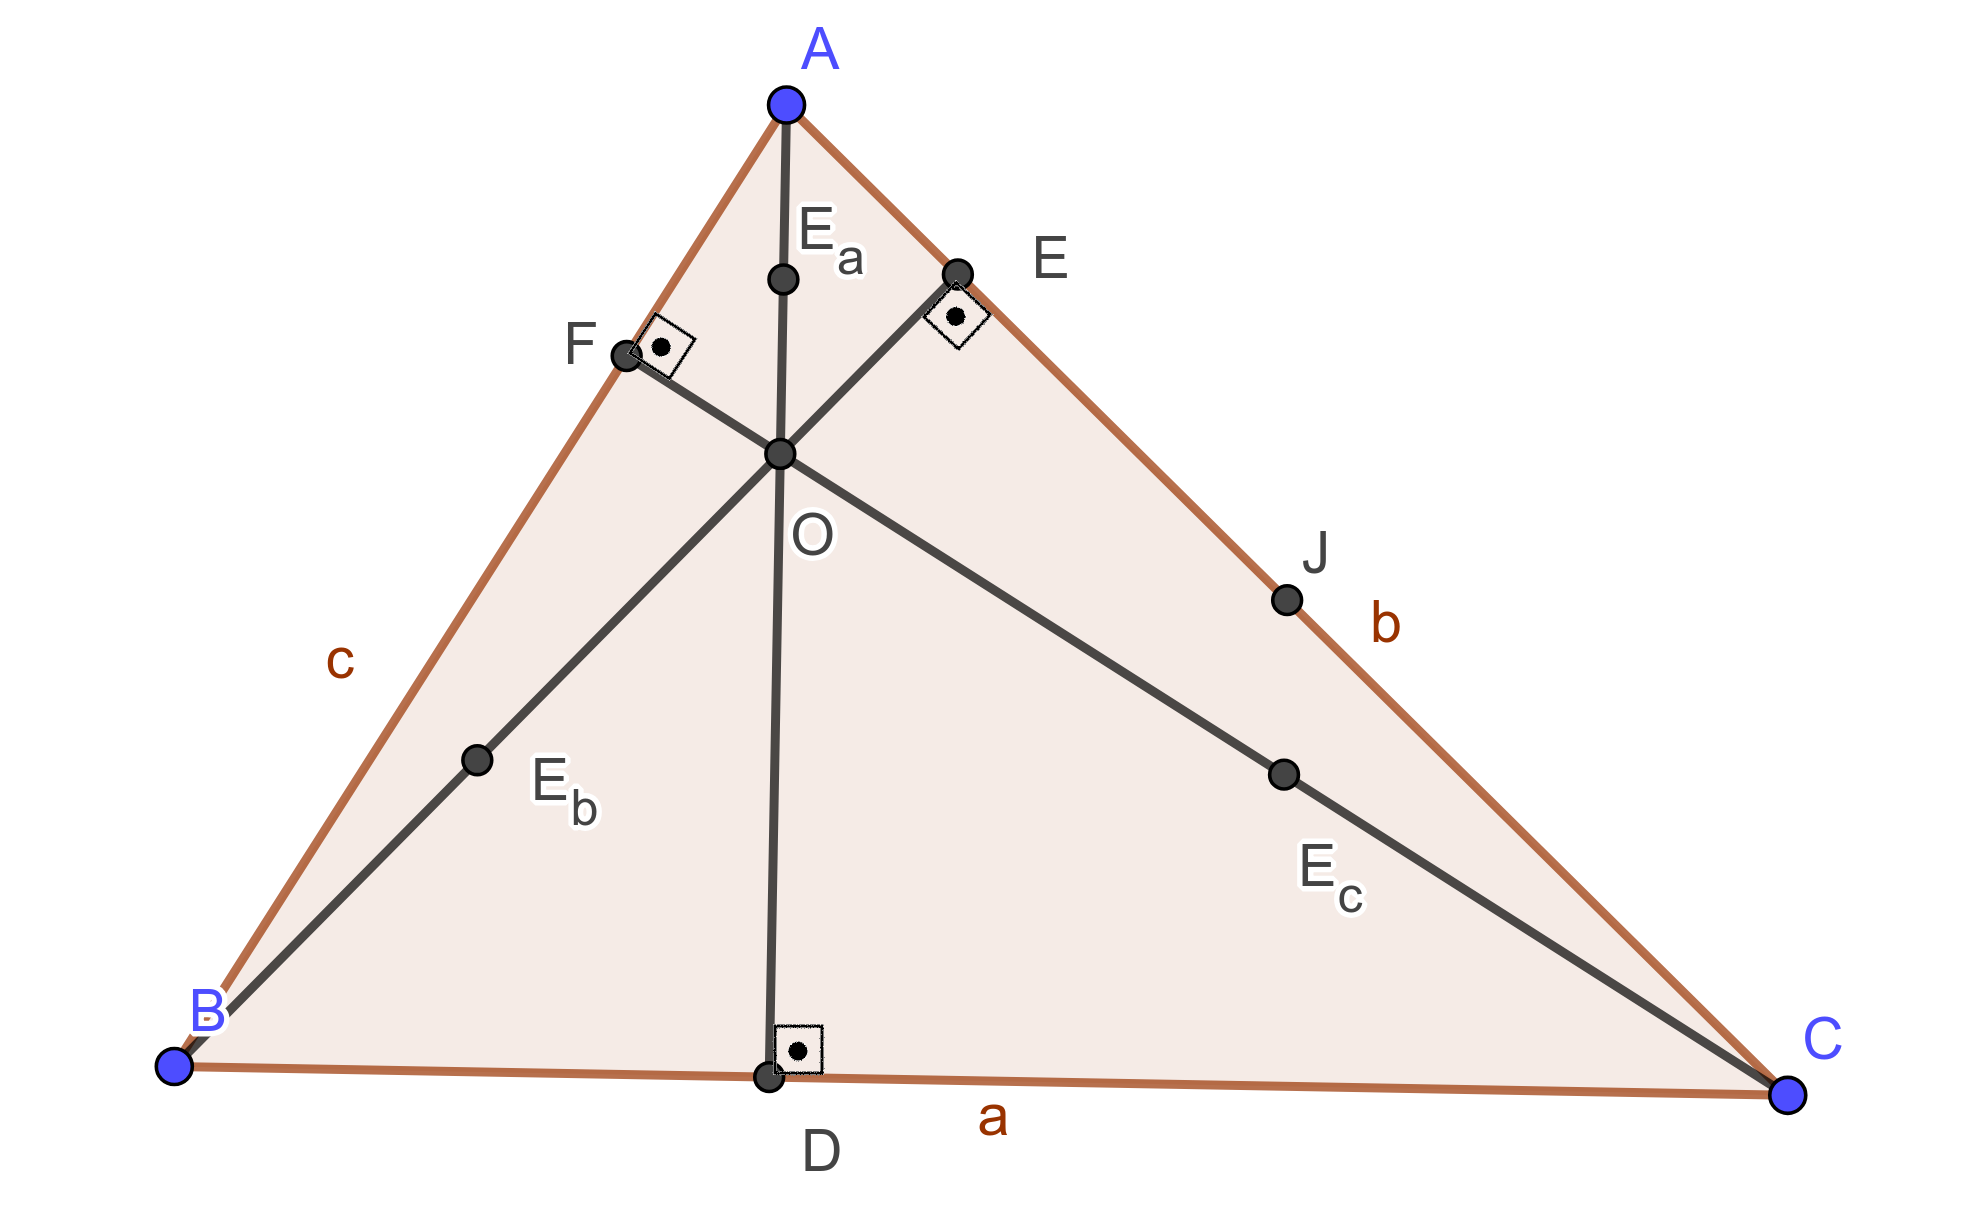
\includegraphics[width=6.9cm]{triangulo4.png}
    \caption{Alturas relativas e $\triangle DEF$ \label{tria4}}
    
\end{figure}

\chapter{A bissetriz e sua paralela}

Considere o triângulo $\triangle ABC$, com a bissetriz $AT_a$, altura $AH_a$, ponto médio $M_a$ relativo ao lado $BC$ e o ponto de Euler $E_a$, conforme figura \ref{triateo} . Faça um círculo de centro $E_a$ passando por $M_a$ de tal forma que intercepte a reta suporte de $AH_a$ no ponto $P$. Trace a linha $M_{a}P$.

\begin{teo}\label{teo1}
	Em qualquer triângulo $\triangle ABC$ com $H_a$ não coincidindo com $M_a$, o segmento $M_{a}P$ é paralelo a bissetriz $AT_a$
\end{teo}

\begin{figure}[h]
	
	\center
	
	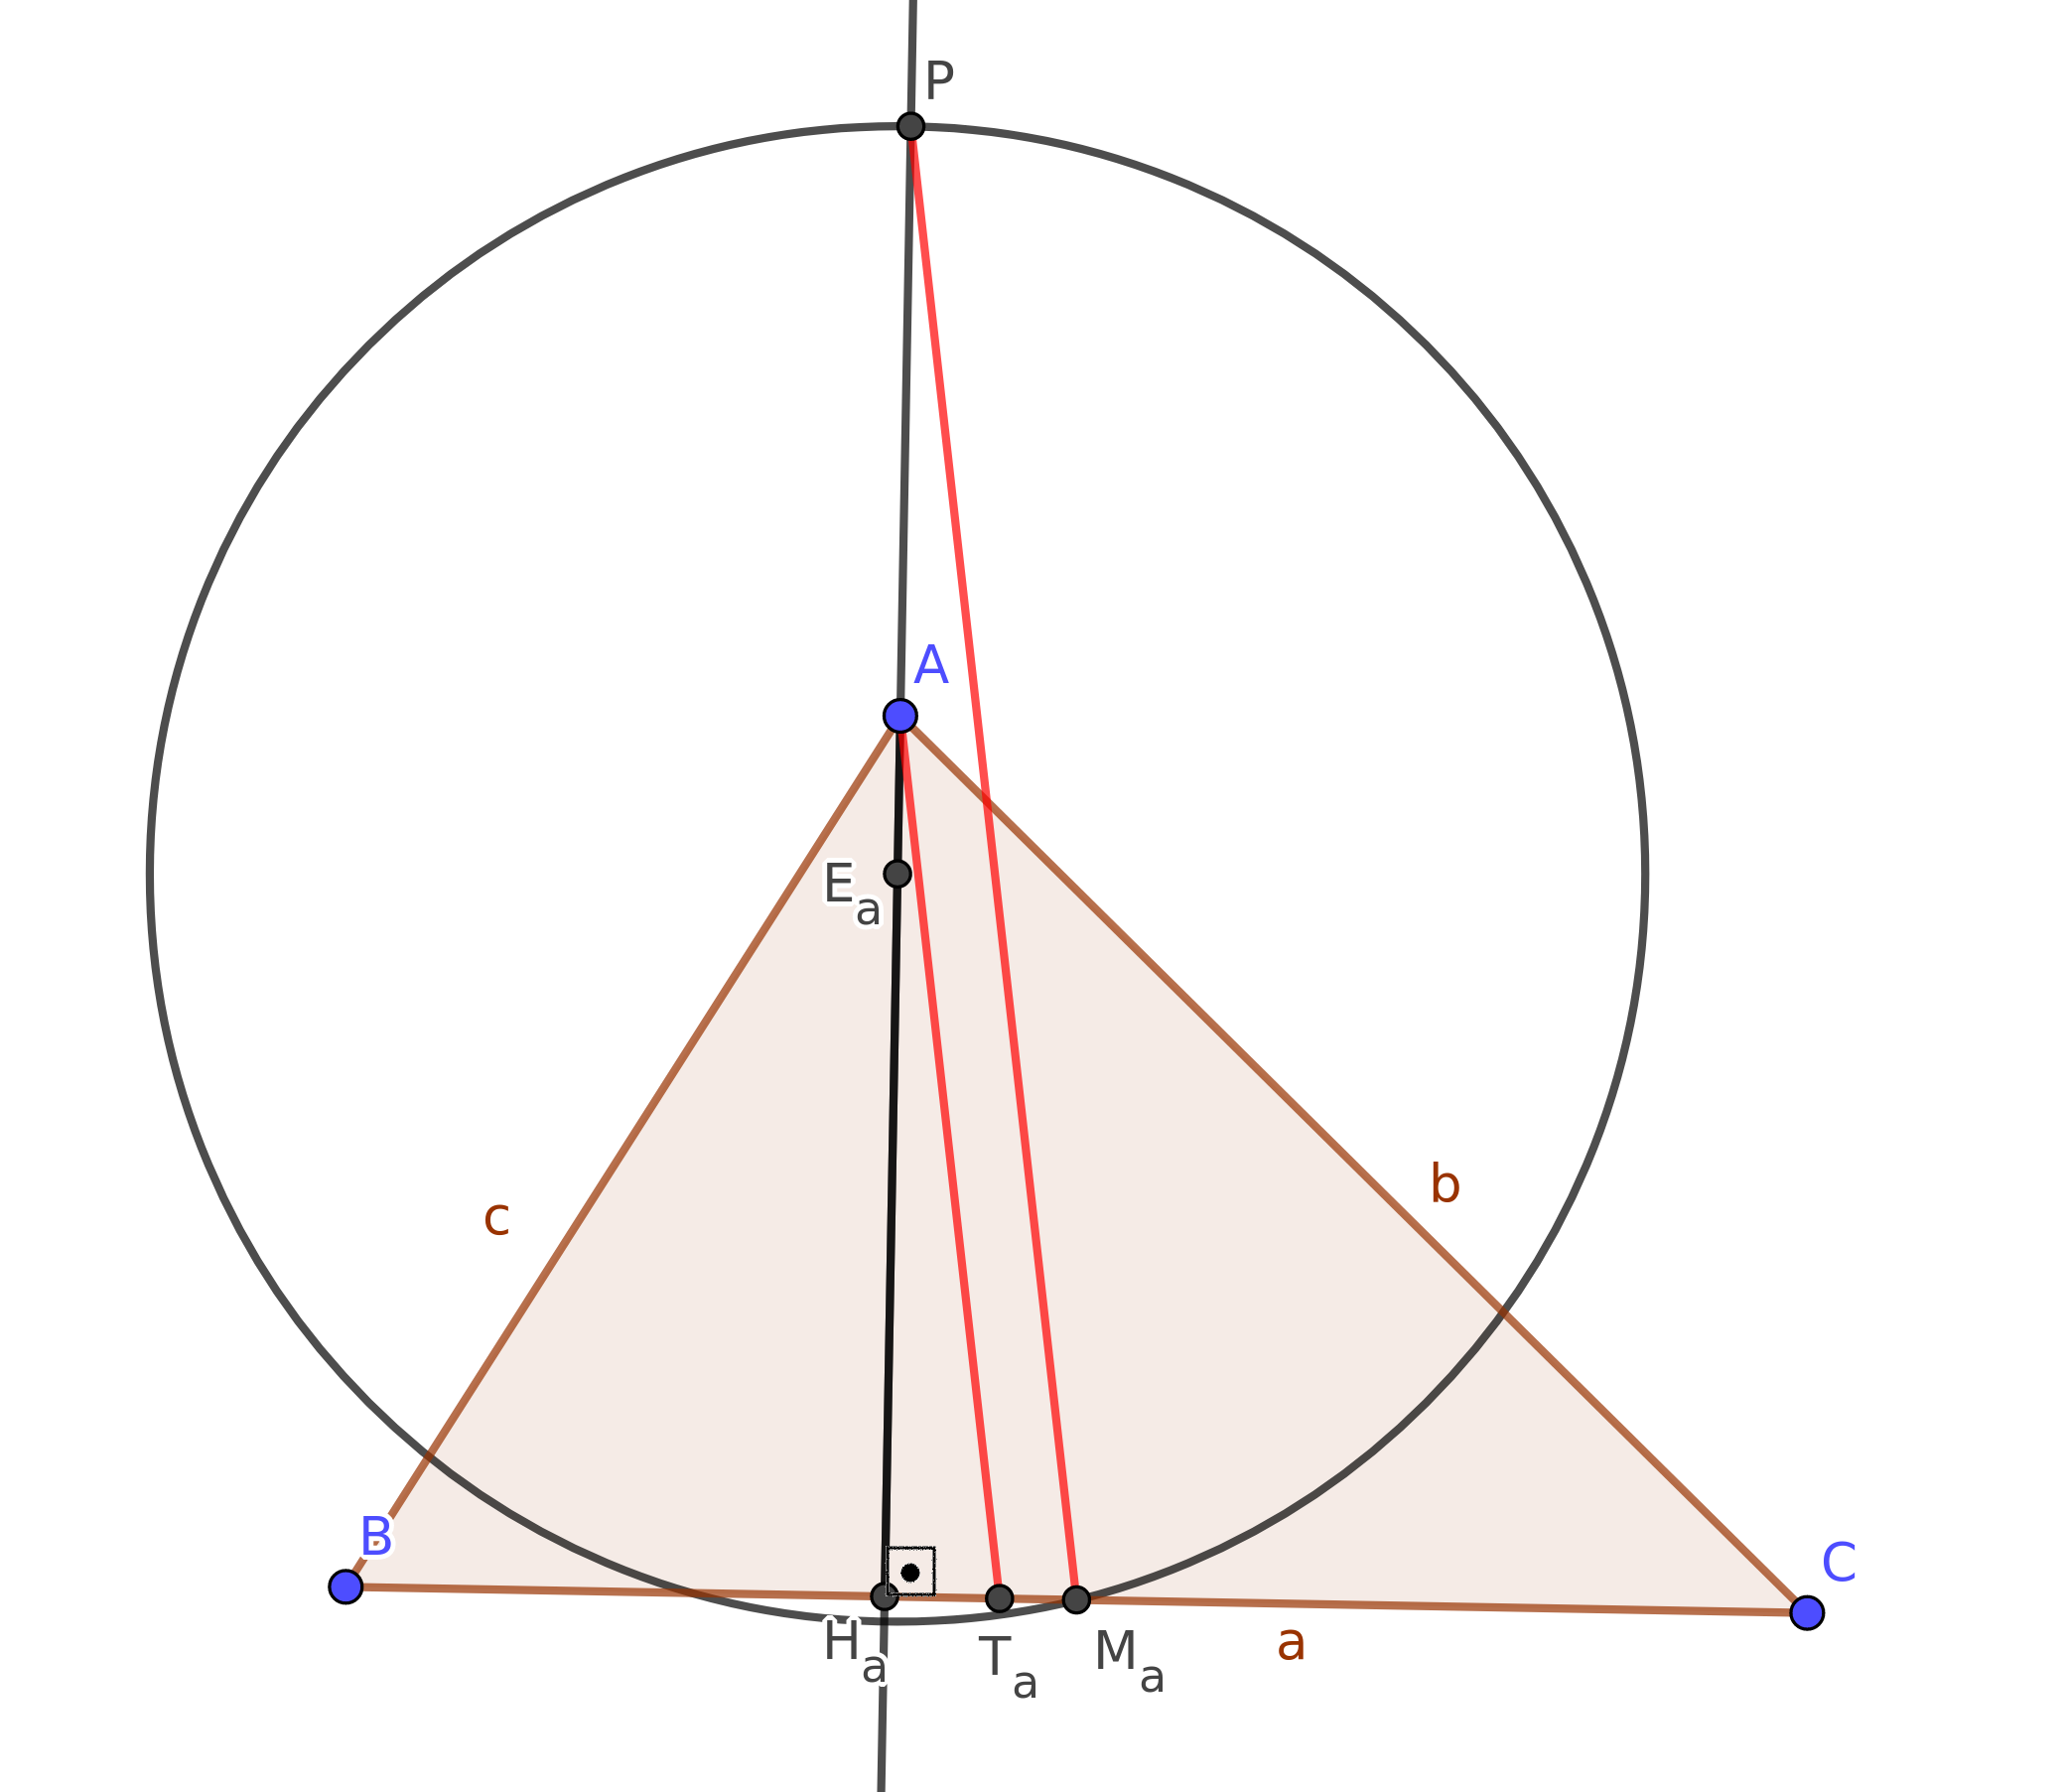
\includegraphics[width=8.5cm]{trianguloteo.png}
	\caption{Bissetriz e sua paralela \label{triateo}}
	
\end{figure}

\textit{Demonstração}

Seja $O$ o circuncentro do $\triangle ABC$. A mediatriz $M_{a}O$ e a bissetriz $AT_a$ intersecta o círculo circunscrito de centro $O$ em $S$, pois vejamos a figura \ref{trianbismed}:

\begin{figure}[h]
	
	\center
	
	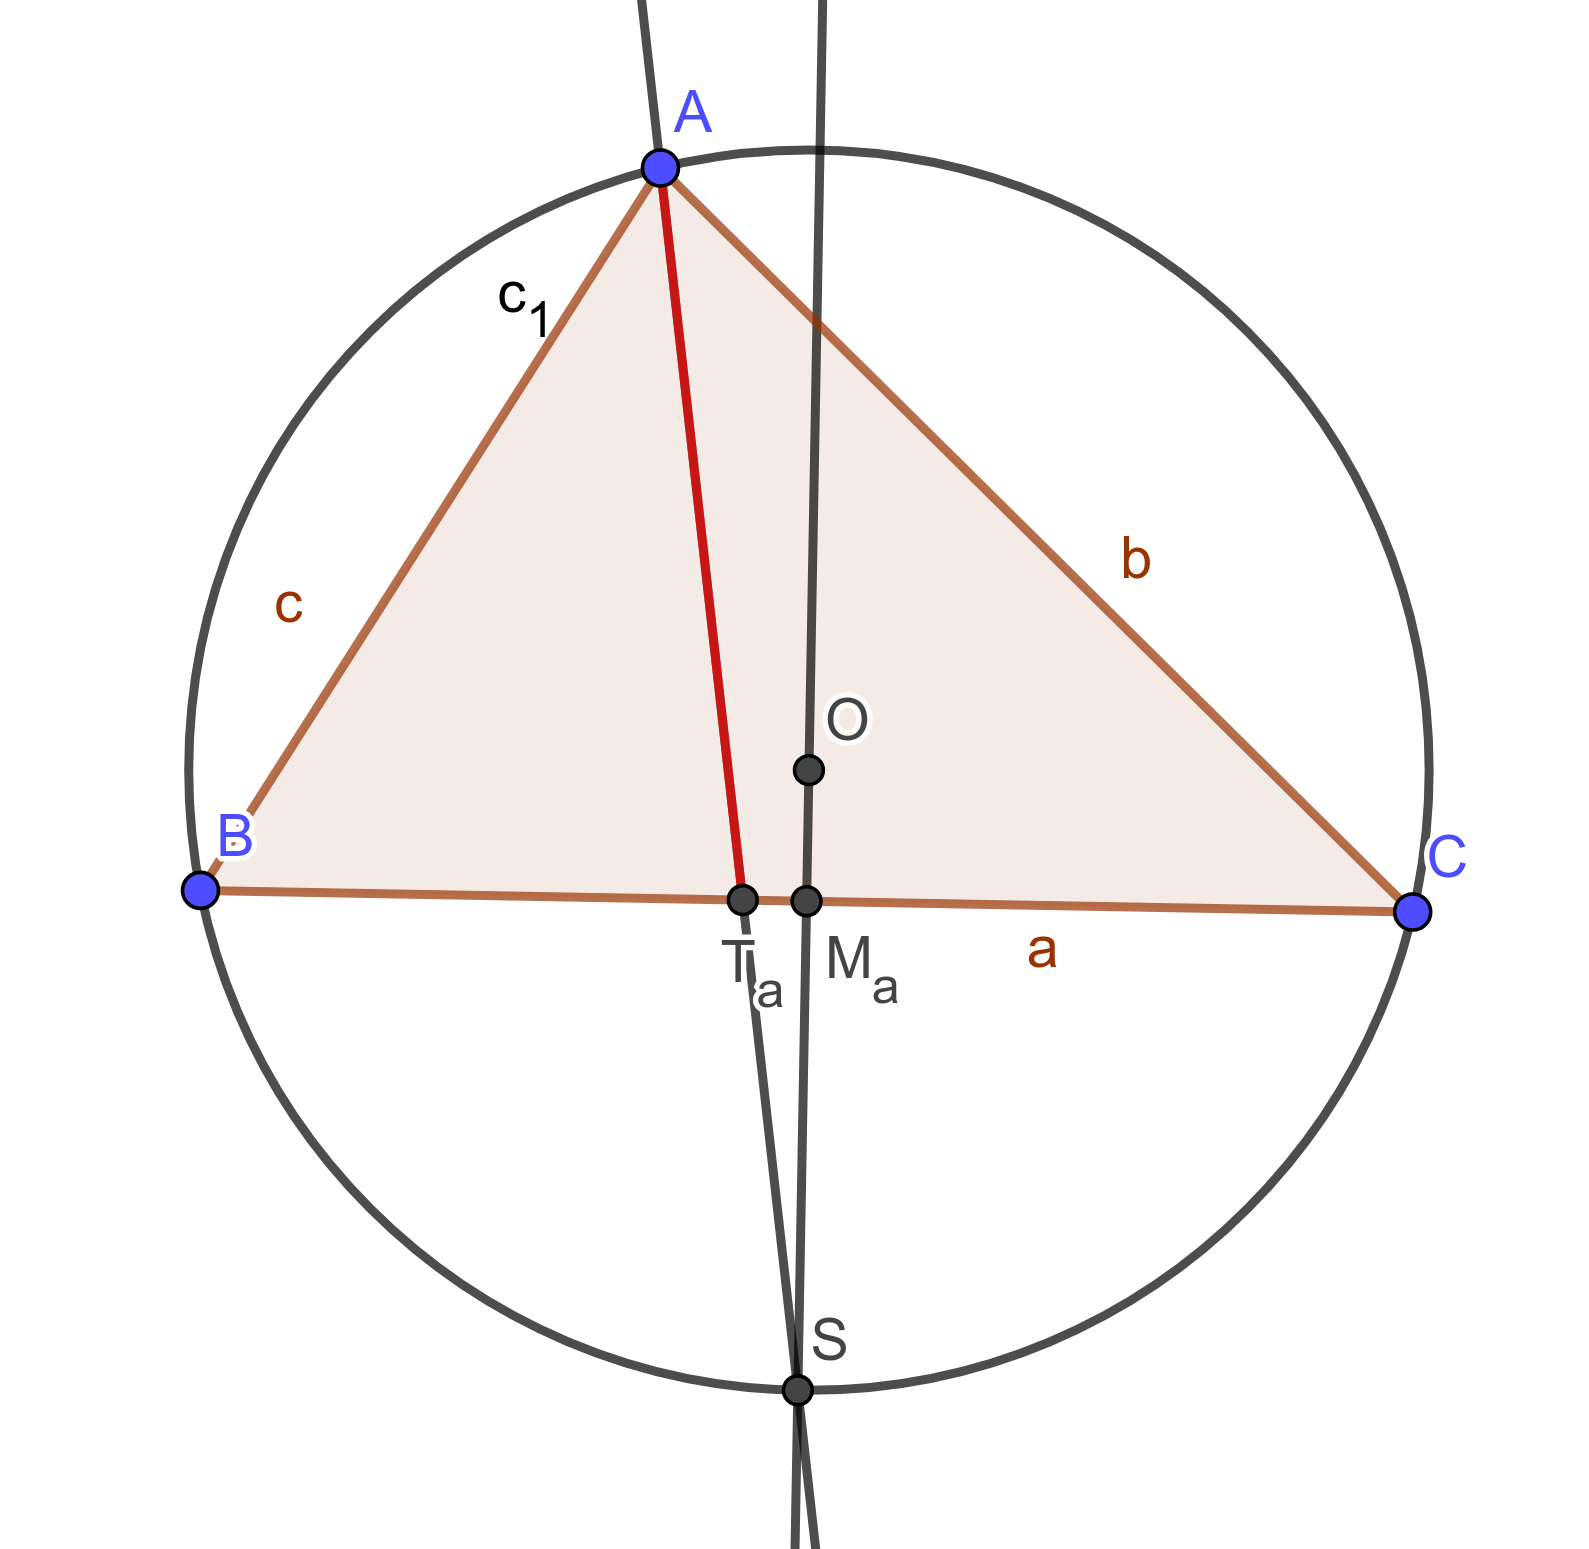
\includegraphics[width=5cm]{triangulocirc.png}
	\caption{Intersecção da bissetriz e da mediatriz\label{trianbismed}}
	
\end{figure}

O ângulo $\hat{BAC}$ tem como arco de visada o arco $BC$. Como $AT_a$ é a bissetriz de $\hat{BAC}$ irá intersectar o círculo de centro $O$ no ponto médio do arco de visada $AB$. A mediatriz $OM_a$ é o lugar geométrico em que todos os pontos estão equidistantes dos pontos $B$ e $C$, logo o ponto em que esta intersecta o círculo de centro $O$ também é equidistante desses pontos, assim também é metade do arco $BC$, logo a mediatriz $OM_a$ e a bissetriz $AT_a$ se intersectam no ponto $S$ contido no círculo de centro $O$.

Agora seja $R$ o ponto médio do segmento $E_{a}O$ e faça a reflexão de toda a figura \ref{trianbismed} com centro em $R$. Seja o  $\triangle A'B'C'$ a reflexão do $\triangle ABC$, conforme a figura \ref{trianref}.

\begin{figure}[h]
	
	\center
	
	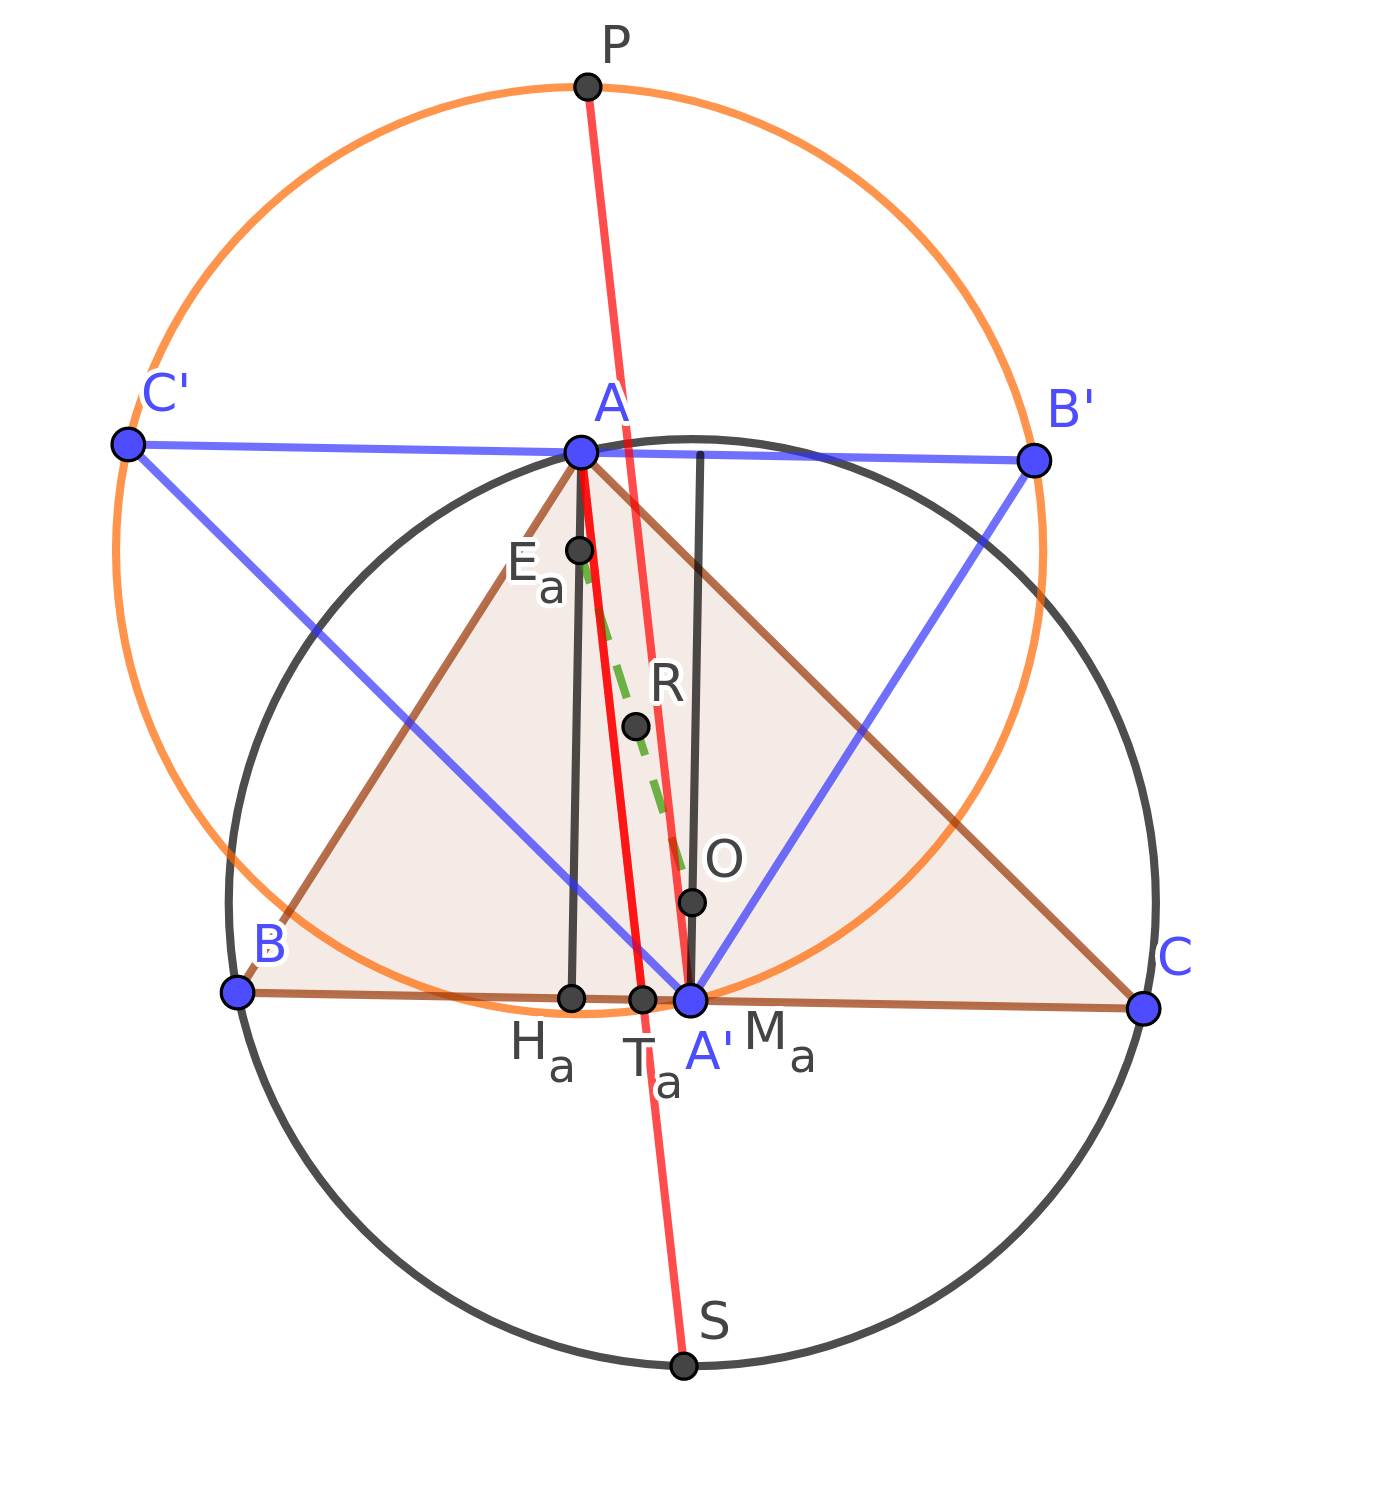
\includegraphics[width=8.5cm]{trianreflexao.png}
	\caption{Reflexão do $\triangle ABC$ \label{trianref}}
	
\end{figure}

Note que, como $R$ é ponto médio de $E_{a}O$, a reflexão de $E_a$ é o próprio ponto $O$ e a reflexão do segmento que passa por $E_a$ saindo do vértice $A$ é o segmento que passa por $O$ saindo de $M_a$, logo o vértice $A'$ coincide com o ponto $M_a$. Desta forma o círculo circunscrito ao $\triangle A'B'C'$ passa também por $M_a$ e tem raio $E_{a}M_{a}$, desta forma, o círculo de centro $E_a$ passando por $M_a$ é a reflexão do círculo circunscrito ao $\triangle ABC$ de centro $O$.

\end{document}
